\chapter{Introduction}
\label{sec:dissertation-thesis}

\section {Dissertation Summary}
Developing a certified loop pipelining algorithm is a complex problem.
We have developed a certified loop pipelining algorithm for behavioral synthesis 
by proper application of theorem proving techniques. The result of this dissertation 
is a framework of certified pipelining primitives which are essential in developing 
any such pipelining algorithm. We systematically build a loop pipelining algorithm 
from ground up using these primitives and certify this algorithm.

\section {Motivation}
Behavioral synthesis~\cite{GMT09,hls-book-2007} is the process of synthesizing an
Electronic System-level (ESL) specification of a hardware
design into a Register-Transfer Level (RTL) implementation.
The idea of ESL is to raise the design abstraction by specifying the high-level,
functional behavior of the hardware design. Designs are
typically specified in a language such as C, C++, or SystemC.
The approach is promising since the user is relieved of
developing and optimizing low-level implementations. 
Studies have shown that ESL 
reduces the design effort by $50\%$ or more while attaining
excellent performance results~\cite{Moussa99}. 
It has recently received significant attention, as the steady 
increase in hardware complexity has made it increasingly 
difficult to design high-quality designs through hand-crafted RTL under 
aggressive time-to-market schedules.  A recent example is VP9 G2 hardware
decoder IP developed by Google~\cite{googledecoder}, which has been implemented primarily in 
standard C++ and synthesized to RTL logic for different target technologies 
and performance points using Calypto's Calatpult High Level Synthesis 
tool~\cite{catapult}. Nevertheless, and in spite of availability of several
commercial behavioral synthesis tools~\cite{ctos,forte,vivado},
the adoption of the approach in main-stream hardware development for
microprocessor and SoC design companies is dependent on 
designers' confidence that the synthesized RTL indeed corresponds to the ESL
specification. 

\begin{figure}[t!]
\begin{center}
\begin{tabular}{c}
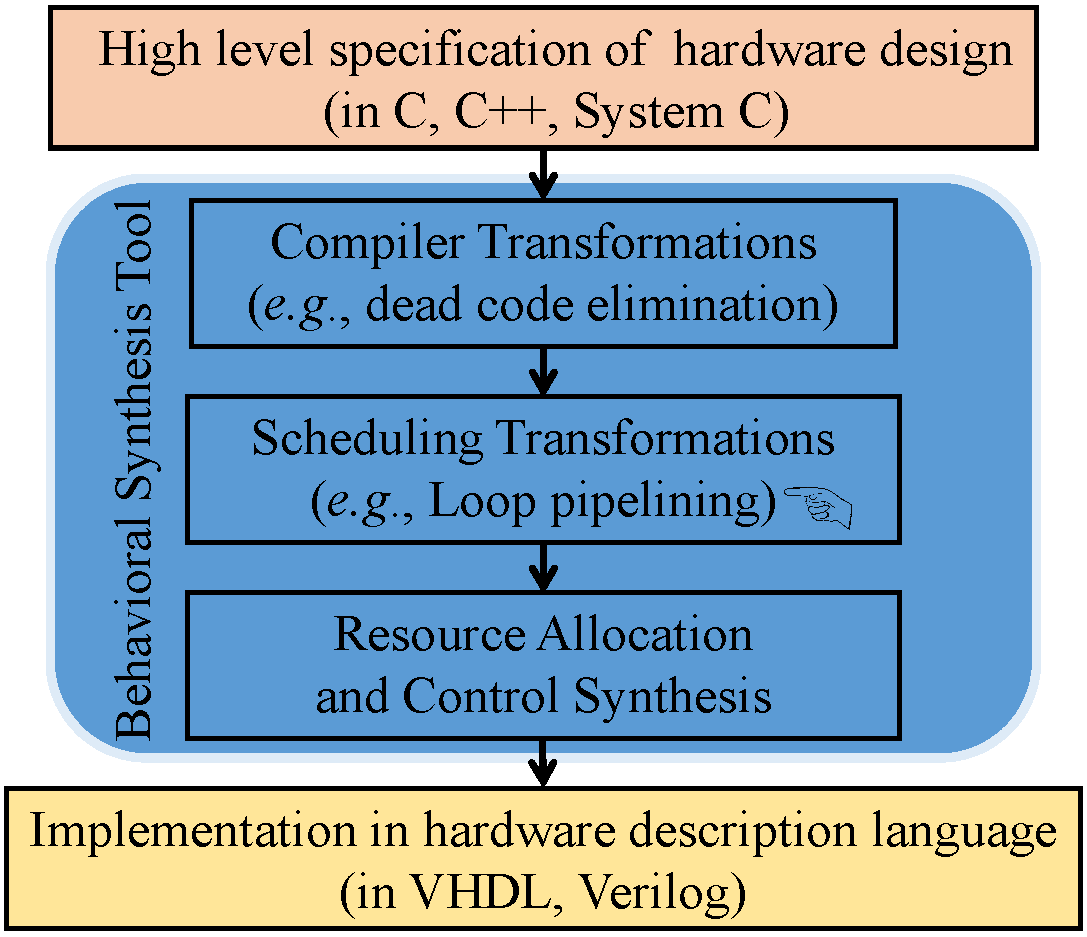
\includegraphics[height=2.8in]{fig-proposal/behavioral-synthesis-intro}
\end{tabular}

\end{center}
\caption{Behavioral Synthesis Flow}
\label{fig:behavioral-synthesis-flow}
\end{figure}

\begin{figure}[t!]
\begin{center}
\begin{tabular}{c}
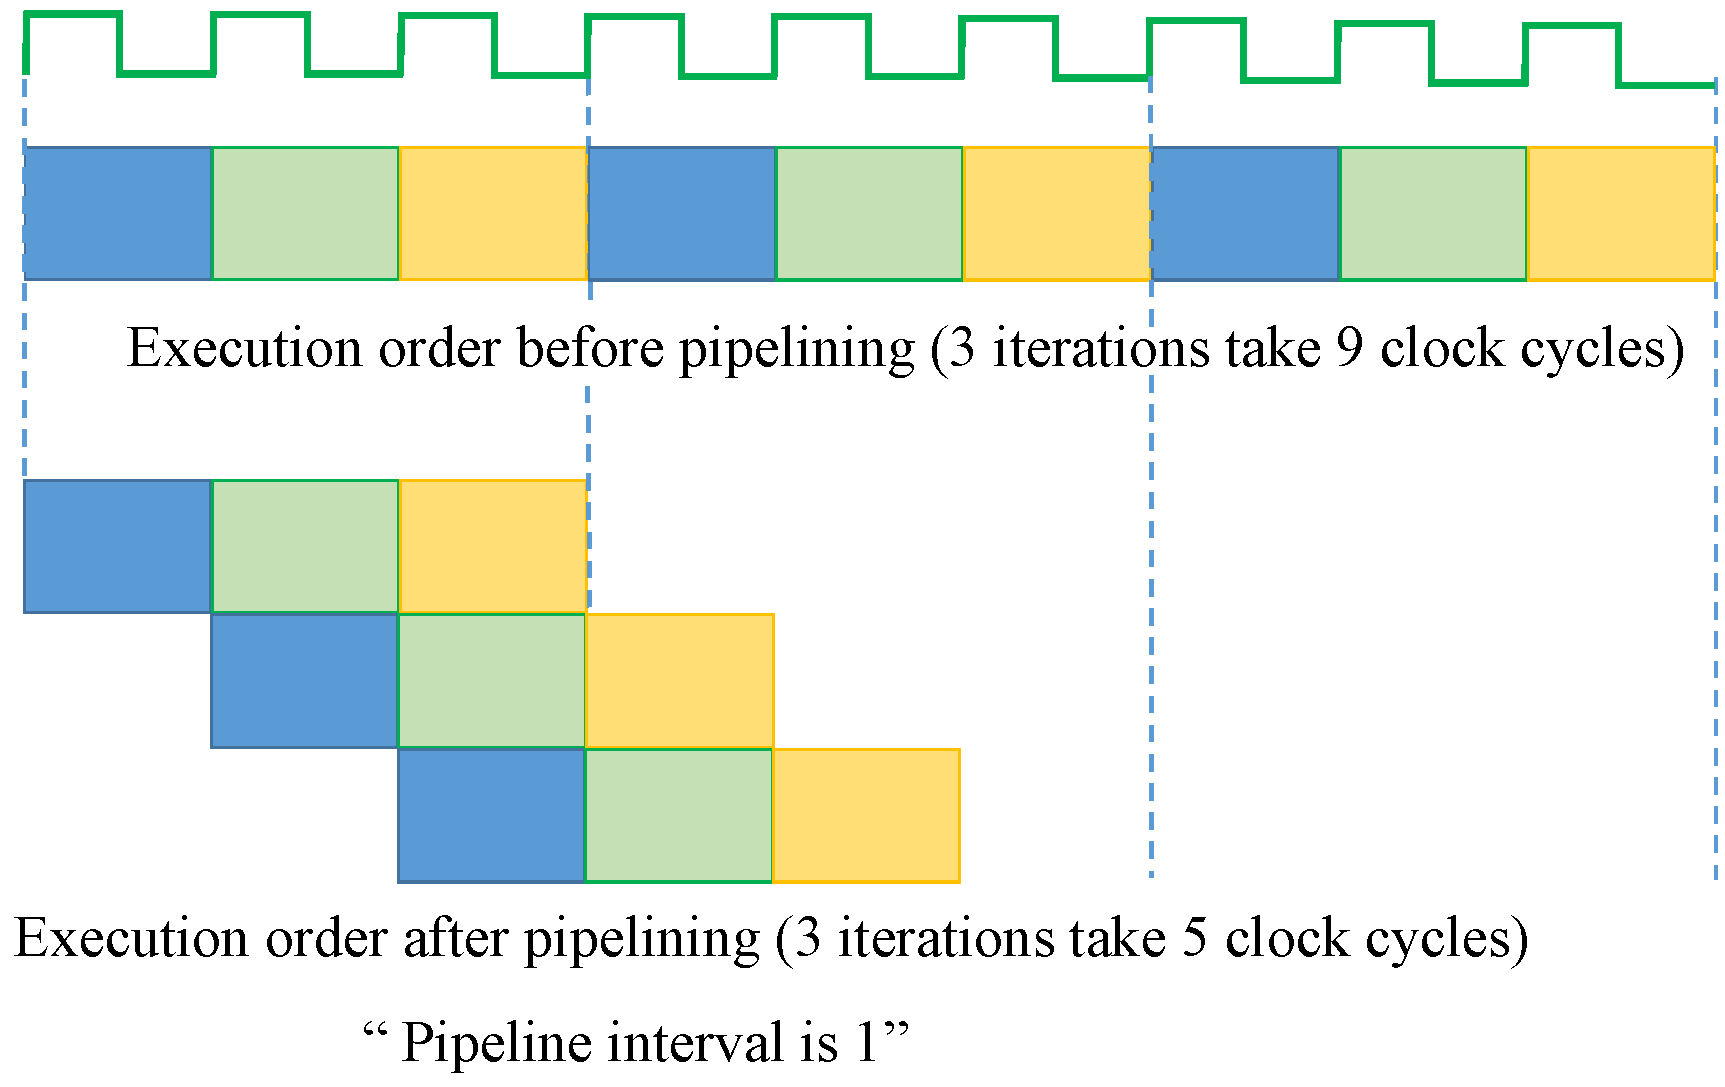
\includegraphics[height=2.8in]{fig-proposal/simple-pipeline}
\end{tabular}
\end{center}
\caption{Loop Pipelining}
\label{fig:simple-pipeline}
\end{figure}

To satisfy the power and performance demands
of modern applications, a behavioral synthesis tool applies
hundreds of transformations. As shown in Figure~\ref{fig:behavioral-synthesis-flow}, 
a typical behavioral synthesis flow can be roughly divided into three phases: 
compiler transformations; scheduling transformations and 
resource allocation and control synthesis. 
Commercial
synthesis tools are highly complex software involving
thousands to millions of lines of code; furthermore, they
perform aggressive optimizations on the design being
synthesized to satisfy constraints on power, performance,
and area.  Tools of such compelxity invariably contain
subtle bugs, which undermine the very effectiveness of
behavioral synthesis.  Consequently, it is critical to
develop a methodology for certifying synthesis
transformations.
%Many of these transformations  involve complex and aggressive optimizations that require subtle and delicate
%invariants. Therefore, it is not surprising that these transformations contain bugs, which can result in errors in synthesized hardware.  
Thus it is critical to develop mechanized support
for certifying the equivalence between ESL and RTL
designs. However, the large difference in
abstraction between the two representations makes such
certification non-trivial.

Loop pipelining is a critical transformation in behavioral
synthesis. The goal of this transformation is to increase
throughput and reduce latency of the synthesized hardware by
allowing temporal overlap of successive loop iterations. 
As shown in Figure~\ref{fig:simple-pipeline}, the three iterations of
overlapped pipeline structure takes only five clock cycles as opposed to 
nine clock cycles if executed sequentially.  It
is performed by most state-of-the-art 
synthesis tools~\cite{forte,vivado,legup}.

Unfortunately, it is also highly complex~\cite{tl:software-popl10} and
error-prone, requiring subtle analysis of invariants to
preclude data hazards arising from overlapping control/data flow of
executions of successive loop iterations.  Furthermore,
certifying the result of this transformation is very
difficult.  In particular, the pipelined output design from
the transformation has a markedly different control/data
flow structure from the sequential design that is input to
the transformation; this makes it hard to find corresponding
internal signals to serve as cutpoints, making it hard to
compare them through sequential equivalence checking.  On
the other hand, applying theorem proving to certify the
pipelining transformation is clearly cost-prohibitive given
the complexity of the implementation; furthermore, most
commercial transformation implementations are proprietary,
making it infeasible to develop such a framework from a
methdological perspective.
As a result, hardware designers are vary of using current behavioral synthesis tools as
they are often deemed either (a) aggressively optimized but error-prone or (b) 
reliable but overly conservative, thus often producing circuits of poor quality
or performance~\cite{spark,kundu2008}. Therefore, ensuring
correctness of behaviorally synthesized pipeline designs
is a critical issue in bringing behavioral synthesis into practice.

An approach for certifying loop pipelining transformations using a combination of SEC and 
theorem proving techniques has been proposed by Hao et al.~\cite{hrx:dac-12}. The most critical and complex
component of their approach (c.f. Section~\ref{subsec:reference-pipeline}) is developing
a loop pipelining algorithm with two key properties: (1) it generates a reference pipeline model 
by exploiting pipeline generation information from the synthesis flow (e.g., the iteration interval 
of a generated pipeline) and the reference model can be compared with a pipelined RTL 
implementation using SEC effectively, and (2) it can be mechanically verified to correctly preserve the semantics of
sequential (non-pipelined) specification of loop execution. Hao et al. showed viability of 
their approach by comparing pipeline generated from their algorithm with RTL implementation 
using SEC. However, their algorithm was not certified as well as incomplete as explained 
later in Section~\ref{subsec:reference-pipeline}. Certification is a key component 
without which correctness of behavioral synthesis process for pipelined designs cannot be claimed.
Therefore, this dissertation on 
developing a certified loop pipelining algorithm using our framework of certified 
primitives is important to facilitating formal verification of behaviorally synthesized
 pipeline designs.

\section{Problem Statement}
Certifying an algorithm especially as complex as loop pipelining is not easy by any known conventional methods. To develop a certified loop pipelining algorithm in behavioral synthesis, we need to address the following key challenges brought about by the semantic gap between the sequential and pipelined designs.

\begin{figure}[t!]
\begin{center}
\begin{tabular}{c}
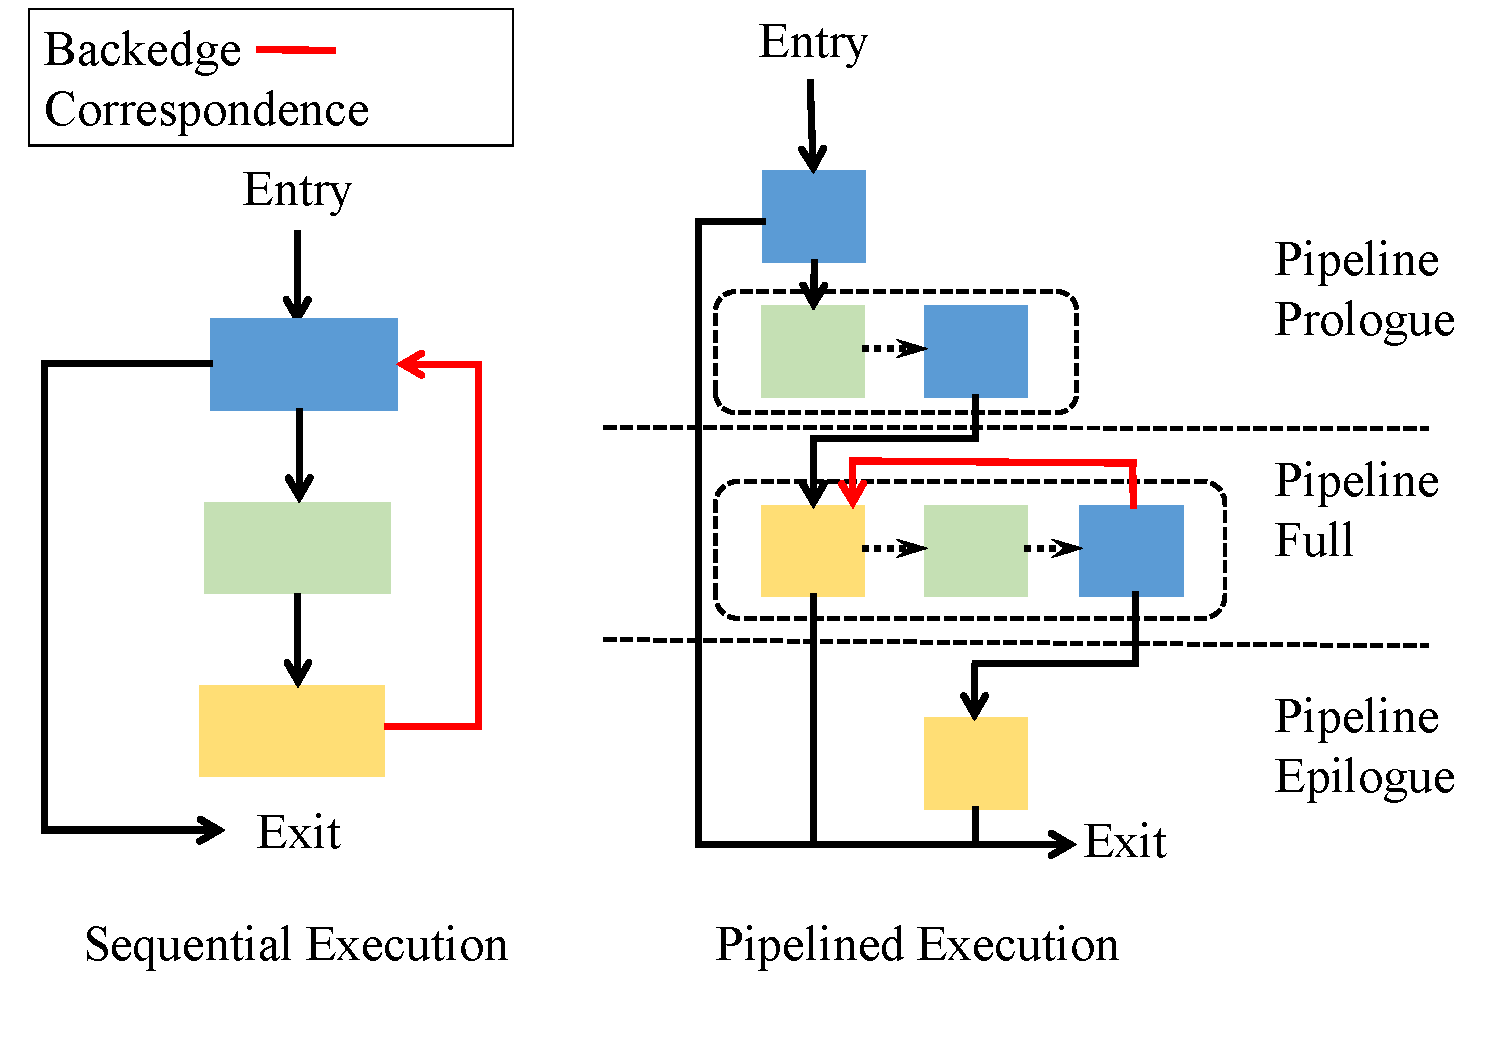
\includegraphics[height=3.3in]{fig-proposal/seq-and-pp}
\end{tabular}
\end{center}
\caption{Back-edge in Sequential Loop Vs Back-edge in Pipelined Loop}
\label{fig:seq-and-pp}
\end{figure}

\begin{enumerate}[--]
\item {\em Formalizing an invariant that links loop in a sequential design with loop in the corresponding pipelined design.} As shown in Figure~\ref{fig:seq-and-pp}, a sequential loop executes its iterations in sequence. The previous loop iteration is complete before the next iteration. A pipelined design, however, overlaps the consecutive iterations of a given design based on pipeline interval. As a result, a loop in the pipelined design executes statements from different iterations of the corresponding sequential loop design. Identifying a provable inductive invariant that links the backedge in the sequential loop with the backedge in the pipelined loop is, therefore, a major challenge.
\item {\em Identifying and certifying underlying primitives in a loop pipelining algorithm.} Certifying a loop pipelining algorithm requires a complex invariant to prove that executing a sequential loop is equivalent to executing a pipelined loop. Identifying the pieces which would make this certification managable is a difficult task. We decompose the algorithm into certifiable primitives. We prove that if each primitive maintains an invariant that the execution of the intermediate representation before and after application of the primitive is same, we can prove that the algorithm also maintains the invariant. This approach, however, requires a crisp understanding of the essential steps involved in developing a pipeline loop from a sequential loop. We need to succinctly identify primitives which maintain the given invariant and are also certifiable by theorem proving. Each primitive would require a systematic approach for its proof.
\item {\em Identify and maintain control flow by proper placement of branches.}  Branch conditions dictate the control flow. Presence of conditional and unconditional branch instructions in a loop means that the loop is no longer executed in a straight line. At each application of primitive, we need to ensure that this control flow is not disturbed or is atleast well accounted for. 
\item {\em Certifying the complete loop pipelining algorithm based on certified primitives.} Although, the primitives act as backbone for our algorithm, their certification alone does not automatically certify the entire algorithm. We need to identify the conditions under which a primitive is correct and make sure that every application of the primitive in the algorithm has the required assumptions.
\end{enumerate}

\section {Overview of our Approach}

\begin{figure}[t!]
\begin{center}
\begin{tabular}{c}
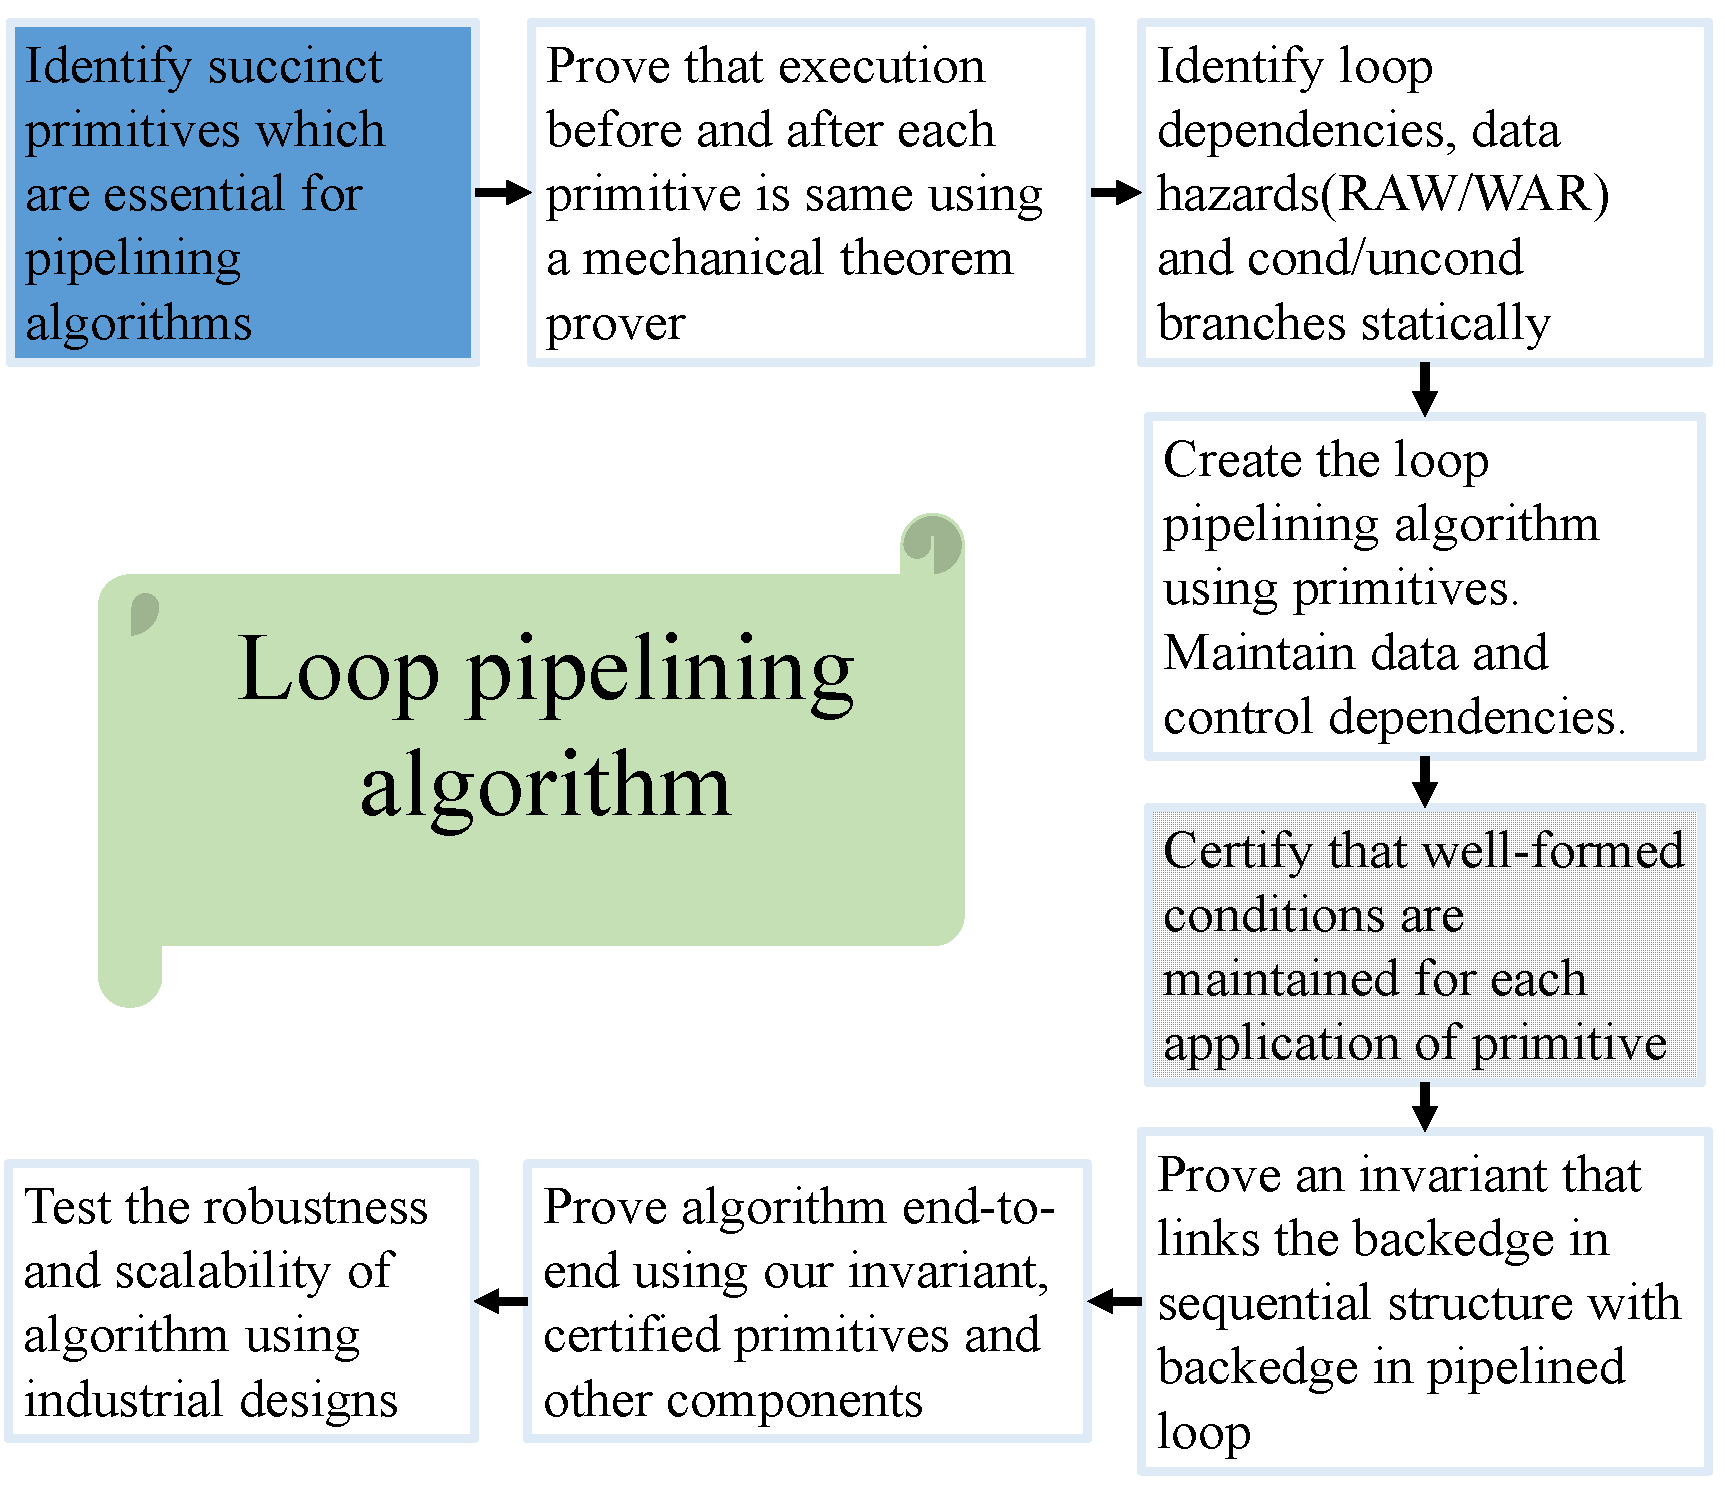
\includegraphics[width=4.75in]{fig-proposal/our-approach}
\end{tabular}
\end{center}
\caption{Overview of our Approach}
\label{fig:our-approach}
\end{figure}

Our work shows that a certified loop pipelining algorithm can be developed by systematic application of theorem proving techniques. 

We have basically divided our approach into eight broad steps as shown in Figure~\ref{fig:our-approach}. The first two steps define our framework of certified primitives which we believe are essential for any certified pipelining algorithm. We have identified these primitives based on a realization that in order to generate a pipelined loop design from a sequential loop design, there are three broad steps: (1) identification and removal of data hazards, (2) overlapping the executions of subsequent iterations after the removal of data hazards, and (3) maintaining the correct control flow to preserve the exit condition and state at the time of exit from the loop. Our primitives are such that they can be applied alone or in combination with other primitives to remove data hazards, reason about branches and to overlap iterations. We certify each primitive by proving that execution before and after each primitive is correct. Certification of each primitive requires separate careful reasoning in a mechanical theorem prover which we describe later in Chapter~\ref{sec:proof}. We have defined the syntax and semantics of intermediate design representation in ACL2~\cite{car,acl2-sandip}. We have formalized and certified all of our primitives in ACL2 theorem prover.
 
The next six steps are for creating the certified loop pipelining algorithm using our framework of certified primitives. Certifying an application of a primitive in the context of the algorithm further involves ensuring that addition of any primitive does not alter the underlying assumptions in the syntax, for example, if we assume there are no return statements in a given representation, applying any primitive should also maintain that assumption. We use these primitives as a backbone to build our loop pipelining algorithm with distinct decomposable components one step at a time. Besides primitives, there are also additional components in the algorithm such as for identifying data hazards and for unrolling the loop. Each component satisfies the invariant that execution of intermediate representations before and after the component is same.  We elaborate on our approach later in Chapter~\ref{sec:pipelining-algorithm}.

We have also identified a unique invariant which proves that executing overlapped iterations is equivalent to executing sequential iterations. It differs from a typical invariant used for correctness of pipelined systems in that it explicitly specifies the correspondence between the sequential and pipelined programs at each transition.  We elaborate on our invariant in Chapter~\ref{sec:proof}. We have proved that our algorithm satisfies this invariant.

We have certified the algorithm end-to-end which means that given a well-formed pipelinable loop (definition explained later in Chapter~\ref{sec:pipelining-algorithm}), we show that executing a sequential loop is equivalent to executing the pipelined loop created using our algorithm. We elaborate on the proof in our proof sketch in Chapter~\ref{sec:proof}. Our proof sketch shows that our primitives are sufficient and essential and that we can build a complete certified loop pipelining algorithm from ground up using our framework.

The major \textbf{contributions} of our dissertation are:
\begin{enumerate}[--]
\item Identifying the key provable primitives essential in pipelining algorithms for behavioral synthesis and certifying these primitives in ACL2 theorem prover;
\item Formalizing an invariant to link the sequential loop before pipelining with the pipelined loop;
\item Developing our own executable loop pipelining algorithm in ACL2 using those primitives and certifying this algorithm using ACL2 theorem prover;
\item Testing our certified loop pipelining algorithm on industrial-strength designs
\end{enumerate}

\section {Outline}
The remainder of this dissertation is organized as
follows. Chapter~\ref{sec:background} provides background on the overall project and 
explains the context of our theorem proving work. Chapter~\ref{sec:formalization} 
discusses our formalization of the intermediate representations used in behavioral synthesis.
We also discuss the correctness statement for loop pipelining algorithms. Chapter~\ref{sec:challenges} 
discusses an earlier proposed algorithm and how and why we have chosen a different approach.
Chapter~\ref{sec:pipelining-algorithm} discusses our framework and a certified loop pipelining 
algorithm we have developed using the framework. Chapter~\ref{sec:proof} provides a proof 
sketch for our algorithm. Chapter~\ref{sec:SEC} provides evaluation of robustness and 
scalability of our algorithm on industrial-strength designs. The related work is discussed in Chapter~\ref{chapter:related-work}.
We then conclude with the major 
contributions of this dissertation and future work in Chapter~\ref{sec:research-plan}.
